\documentclass[main]{subfiles}
\usepackage[sols]{workbook}
\numbering{ws3-8}

\begin{document}

\ifSubfilesClassLoaded{%
  \chaptermark{\chapterthree}
}{}

\section{Systems of First-Order Differential Equations} \label{ws3-8}

\begin{framed}
\centerline{\textbf{Lesson Goals}}

You should be able to:
\begin{itemize}
\item Interpret basic systems of first-order differential equations, and check whether a given pair of functions is a solution to a system
\item Make sense of the phase plane for a system of a first-order differential equations, and plot basic solution trajectories in the phase plane
\item Compare and contrast the phase plane for a system with the normal graphs of the solution functions, and sketch one graph given the other
\end{itemize}
\end{framed}
%\end{comment}

\begin{enumerate}

  

\item   \label{reaction-irreversible}

\note{I'll ask the students to try this problem and then we'll discuss it as a
class.  Part (a) really helps in drawing the solution trajectory.  I'll also use
the final part of this problem to introduce the concept of {\em equilibrium}
solutions.  An equilibrium is a {\em pair} of constant functions (one for $A$
and one for $B$) that simultaneously satisfy both DEs.  This system has infinitely
many equilibria, but only one that satisfies the given ICs.}

This problem concerns a simple decay process by which molecules of chemical $A$
spontaneously and irreversibly decay\footnote{For example, you can think of
radioactive decay of carbon-14 to nitrogen-14.} to chemical $B$ in
a closed, isolated sample.
Assume that the rate of decay of $A$ in a sample is proportional to the amount
of $A$ in the sample.  This situation is modeled by the system
$$
  \frac{dA}{dt} = -kA \qquad \frac{dB}{dt} = kA.
$$ 
Chemists would indicate such a reaction schematically using
the notation $A \xrightarrow{k} B$, where the proportionality constant $k > 0$ is
known as a {\em kinetic constant}.

\begin{enumerate}

  \item
  \begin{problem}[1in]
    Explain, both in mathematical terms and chemistry terms, why $A(t) + B(t)$ must
    remain constant.  Hint:  Add the two differential equations.
  \end{problem}

  \begin{solution}
    Notice that $\displaystyle \frac{dA}{dt} + \frac{dB}{dt} = -kA + kA = 0$.  We also
    know by the ``sum rule" for differentiation that 
    $\displaystyle \frac{dA}{dt} + \frac{dB}{dt} = \frac{d}{dt} (A + B)$.  But if
    $\displaystyle \frac{d}{dt} (A + B) = 0$, this means that $A + B$ must remain constant.
    This make sense on chemistry grounds:  if the sample is closed and isolated, then
    the total amount of $A$ and $B$ must remain constant---every decay of one
    molecule of $A$ results in a gain of one molecule of $B$.
  \end{solution}

  \item
  \begin{problem}[1in]
    Suppose that, from empirical measurements, we have $k = 2$, and that the initial
    amounts of $A$ and $B$ in a sample are $A(0) = 10$ and $B(0) = 0$.  Find the solution
    of the system of differential equations that satisfies these conditions. 
  \end{problem}

  \begin{solution}
    With $k = 2$, the differential equations are $dA/dt = -2A$ and $dB/dt = 2A$.
    The differential equation for $A$ is one that we recognize and have seen many times:
    its general solution is $A = C e^{-2t}$ where $C$ is a constant.  Since $A(0) = 10$,
    we find that $C = 10$, and therefore \fbox{$A(t) = 10 e^{-2t}$}.  

    To find $B(t)$, one option is to substitute this formula into the $dB/dt$ equation
    and solve for $B$ by integrating.  But the result of Part (a) will save us lots of
    work---we know that $A(t) + B(t)$ must remain constant.  In particular, $A(t) + B(t)$
    must equal $A(0) + B(0) = 10$.  This means that $A(t) + B(t) = 10$ for all time $t$,
    and therefore \fbox{$B(t) = 10 - 10e^{-2t}$}.
  \end{solution}
\pspace{\newpage}
  \item
  \begin{problem}[7in]
    Consider the pair $A(t)$, $B(t)$ you found in Part (b).  Give three plots:
    $A(t)$ versus $t$, $B(t)$ versus $t$, and a phase plane plot of the solution
    trajectory (i.e., a parametric plot of $B(t)$ versus $A(t)$).
  \end{problem}

  \begin{solution}
    The graph of $A(t)$ versus $t$ is simply a decaying exponential function.
    The solution trajectory in the phase plane (rightmost panel in the figure below)
    is a straight line of slope $-1$.  Indeed, $A + B = 10$ for all time $t$,
    and the graph of $B = 10 - A$ forms a straight line of slope $-1$.
\begin{center}
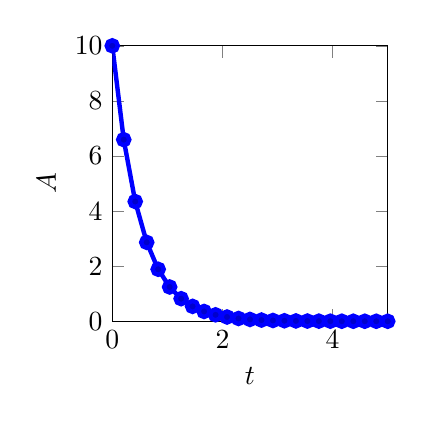
\begin{tikzpicture}
\begin{axis}[
%axis lines = middle,
            width=2in,
            height=2in,
            xlabel=$t$,
            ylabel=$A$,
            %ytick={0,1, 2},
            ymin=0,
            xmin=0,
            xmax=5,
            ymax=10
            ]   
\addplot+[blue, ultra thick, domain={0:5}]{10*exp(-2*x)};
\end{axis}
\end{tikzpicture}
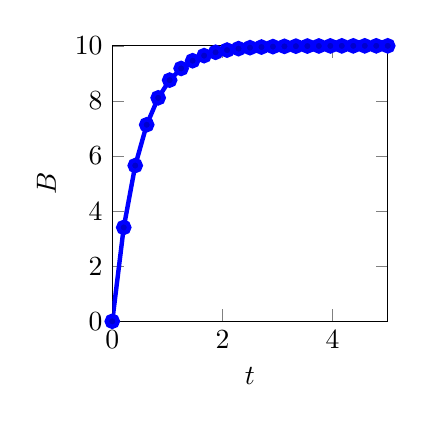
\begin{tikzpicture}
\begin{axis}[
%axis lines = middle,
            width=2in,
            height=2in,
            xlabel=$t$,
            ylabel=$B$,
            %ytick={0,1, 2},
            ymin=0,
            xmin=0,
            xmax=5,
            ymax=10
            ]   
\addplot+[blue, ultra thick, domain={0:5}]{10-10*exp(-2*x)};
\end{axis}
\end{tikzpicture}
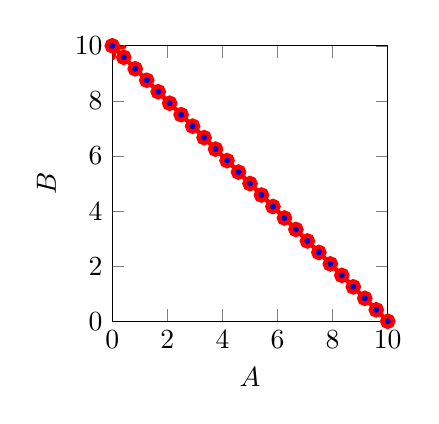
\begin{tikzpicture}
\begin{axis}[
%axis lines = middle,
            width=2in,
            height=2in,
            xlabel=$A$,
            ylabel=$B$,
            %ytick={0,1, 2},
            ymin=0,
            xmin=0,
            xmax=10,
            ymax=10
            ]   
\addplot+[<-, red, ultra thick, domain={0:10}]{10-x};
\end{axis}
\end{tikzpicture}
\end{center}   
  \end{solution}

  \item
  \begin{problem}[\vfill]
    What equilibrium does the pair $A(t)$, $B(t)$ approach as $t \to \infty$?  
  \end{problem}

  \begin{solution}
    As $t \to \infty$, note that $e^{-2t} \to 0$.  This means that $A(t) \to 0$
    and $B(t) \to 10$, which makes perfect sense on chemical grounds---in the long
    run, all of the $A$ molecules will have decayed to $B$.  The system approaches
    the equilibrium $(A,B) = (0,10)$ as $t \to \infty$.

    In general, an {\bf equilibrium} of a system of two differential equations is a 
    pair of constant functions (one for each dependent variable) that simultaneously
    satisfies both differential equations.
  \end{solution}

\end{enumerate}


%%%%%%%%%%%%%%%%%%%%%%%%%%%%%%%%%%%%%%%%%%%%%%%%%%%%%%%%%%%%%%%%%%%%%%
  
  
    \pspace{\newpage}
  
  %\note{I'll have the students work on this one in groups.}

    \item 
  Being deliberately playful, Steve Strogatz (now a professor at Cornell)
  came up with the following system to model the relationship between
  Romeo and Juliet.

  Let $j(t)$ be a measure of Juliet's feelings for Romeo at time $t$, and
  let $r(t)$ be a measure of Romeo's feelings for Juliet, with $t = 0$
  being the time of the Capulet ball where Romeo and Juliet met.  Positive
  values indicate love, and negative values indicate hate.  Then,
  (according to Steve Strogatz, at least), the following system models the
  relationship between Romeo and Juliet:
  \[ \left\{
  \begin{aligned}
  \frac{dj}{dt} &= -r \\
  \frac{dr}{dt} &= j \\
  \end{aligned} \right.\]
  \begin{enumerate}
    \item

    
    \begin{problem}[0.5in]
    According to this model, which of the following statements are true? 
    \begin{enumerate}[topsep=0pt,itemsep=0pt]
    \item The more Romeo loves Juliet, the more Juliet feelings towards him warm.
   
    \item The more Juliet loves Romeo, the more Romeo's feelings for her grow warmer.

    \item Juliet feelings for Romeo warm most rapidly when he loves her least.
    When he loves her most, her feelings are turning sour. 
  \end{enumerate}
  \end{problem}

  \begin{solution}
  In the model, $\frac{dj}{dt} = -r$, so when Romeo loves Juliet ($r >
  0$), her feelings for him decrease.  Thus, the first statement is
  not correct.

  When Juliet loves Romeo ($j > 0$), $\frac{dr}{dt} =j$ is also
  positive, so Romeo's feelings for Juliet increase.  Thus, the second
  statement is true.

  The third statement is also true: $\frac{dj}{dt} = -r$, so
  $\frac{dj}{dt}$ is positive when $r$ is negative, and vice versa. 
  \end{solution}

  \item
  \begin{problem}[0.5in]
  One of the following is the general solution of the system; which
  one?
  \begin{enumerate}[itemsep=0.4in]
    \item $j(t) = - C_1 e^{-t} + C_2 e^t$ and $r(t) = C_1 e^{-t} + C_2
    e^t$.
    \item $j(t) = -C_1 \sin t + C_2 \cos t$ and $r(t) = C_1 \cos t + C_2
    \sin t$.
    \item $j(t) = C_1 \sin t + C_2 \cos t$ and $r(t) = C_1 \cos t + C_2
    \sin t$.
  \end{enumerate}
  \end{problem}

  \begin{solution}
  The correct one is \fbox{ii}, $j(t) = -C_1 \sin t + C_2 \cos t$ and
  $r(t) = C_1 \cos t + C_2 \sin t$.  We can check this simply by
  plugging in.  With these functions, $\frac{dj}{dt} = - C_1 \cos t -
  C_2 \sin t = - r$, and $\frac{dr}{dt} = - C_1 \sin t + C_2 \cos t =
  j$, as we wanted.
  \end{solution}

  \item
  \note{The main thing I want students to understand is that the
  constants $C_1$ and $C_2$ are ``shared'' between $r(t)$ and $j(t)$.}

  \begin{problem}[3in]
  Find the particular solution satisfying $j(0) = 0$ and $r(0) = 1$.
  \end{problem}

  \begin{solution}
  All we need to do is plug the initial conditions into the general
  solution to solve for $C_1$ and $C_2$.
  \begin{itemize}
    \item Since $j(t) = -C_1 \sin t + C_2 \cos t$, the initial condition
    $j(0) = 0$ tells us that $C_2 = 0$.
    \item Since $r(t) = C_1 \cos t + C_2 \sin t$, the initial condition
    $r(0) = 1$ tells us that $C_1 = 1$.
  \end{itemize}
  Therefore, the solution we want is \fbox{$j(t) = - \sin t$, $r(t) =
  \cos t$}.  Notice that a solution consists of \textbf{two}
  functions.
  \end{solution}

\pspace{\newpage}
 
  \item
  \begin{problem}[1in]
  For the particular solution you found in Part (c), graph $j(t)$ and $r(t)$ 
  on the following set of axes.    Describe Romeo and Juliet's relationship 
  over time (using words, not math). 


  \probonly{
\includegraphics[height=1.8in]{ws/images/romeo-juliet-time-axes}}

  \end{problem}

  \begin{solution}
  Since $j(t) = -\sin t$ and $r(t) = \cos t$, here's our graph, with
  $j(t)$ in red and $r(t)$ in blue:
  \begin{center}
  
\includegraphics[height=2in]{ws/images/romeo-juliet-graphs-1}
  \end{center}
  \end{solution}


 %\pspace{\newpage}
  

  \item
  %\note{Some students may see right away that this parameterizes a circle.  I'd like to do it just from looking at where the graphs of $j(t)$ and $r(t)$ are decreasing or increasing because this is a more general method, and it makes the point that places where $j'(t) = 0$ or $r'(t) = 0$ are important.  Students may wonder how accurate such a sketch needs to be.  I tell them that, for now, the important thing is to get the general direction right; by ``general  direction,'' I mean whether the trajectory is going up or down, left or right. (Eventually, we will talk a bit about using $\frac{dr}{dj}$ to find the shape of trajectories, but that's not something we really want them to focus on now.)}

  \begin{problem}
  Sketch the solution you found in Part (c) in the phase plane.

  \probonly{
\includegraphics[height=2.5in]{ws/images/romeo-juliet-axes}} 
  \end{problem}

  \begin{solution}
  Let's use our graphs from Part (d) to do this.
  At time $t = 0$, $j(0) = 0$ and $r(0) = 1$, so our trajectory will
  start at $(0, 1)$.

  Between times $t = 0$ and $t = \frac{\pi}{2}$, $j(t)$ decreases to
  $-1$, and $r(t)$ decreases to $0$.  So, in this time interval, the
  trajectory travels to the left and down, ending up at $(-1, 0)$.

  Between times $t = \frac{\pi}{2}$ and $t = \pi$, $j(t)$ increases to
  0 and $r(t)$ decreases to $-1$.  So, in this time interval, the
  trajectory travels to the right and down, ending up at $(0, -1)$.

  Between times $t = \pi$ and $t = \frac{3 \pi}{2}$, $j(t)$ increases
  to $1$ and $r(t)$ increases to 0.  So, in this time interval, the
  trajectory travels to the right and up, ending up at $(1, 0)$.

  Between times $t = \frac{3 \pi}{2}$ and $t = \pi$, $j(t)$ decreases
  to 0, and $r(t)$ increases to $1$.  So, in this time interval, the
  trajectory travels to the left and up, ending up at $(0, 1)$.

  We are now back where we started, so the cycle just repeats
  forever.  This gives us a picture like:
  \begin{center}
  
\includegraphics[width=2in]{ws/images/romeo-juliet-trajectory-1}
  \end{center}
  (Notice that we have put an arrow on the trajectory to indicate
  time; beyond that, we don't see any information about time when we
  look at the phase plane.)

  Some notes:
  \begin{itemize}
    \item From the description we gave above, we cannot be sure that the
    shape of the trajectory is a circle.  However, since we know from
    Part (c) that $j(t) = - \sin t$ and
    $r(t) = \cos t$, we can see that $j^2 + r^2$ is $(-\sin t)^2 +
    \cos^2 t = \sin^2 t + \cos^2 t$, which is always equal to 1.  So,
    the trajectory does indeed travel along the circle $j^2 + r^2 =
    1$.

    \item In general, the important times to look at are those when
    $j(t)$ or $r(t)$ changes from increasing to decreasing or vice
    versa; these are exactly the times when the trajectory can change
    direction (from, say, going up and right to going up and left).
  \end{itemize}
  \end{solution}

  \item
  \note{An introduction to an equilibrium point.}

  \begin{problem}[2in]
  Suppose that fate prevented Romeo from attending the Capulet ball.
  What initial condition could you then write for the system?  Find
  the particular solution satisfying the initial condition.  Graph it
  like you did in Part (d).  Then, sketch the
  corresponding trajectory on your picture from
  Part~(e).
  \end{problem}

  \begin{solution}
  If they had not met at the Capulet ball, then they would have no
  feelings for each other at that time ($t = 0$), so we would have
  $j(0) = 0$ and $r(0) = 0$.  Plugging these initial conditions into
  the general solution from Part (b), we find
  that $C_1 = C_2 = 0$, so $j(t) = 0$ and $r(t) = 0$.  To graph $j(t)$
  and $r(t)$ as in Part (d), we'd just be graphing
  $j(t) = 0$ and $r(t) = 0$.

  The corresponding trajectory is just a point $(0, 0)$ on the phase
  plane. 
  \end{solution}
\pspace{\newpage}
  \item
  \note{The main point is to have graphs that accurately reflect
  the general direction of the trajectory.  I also emphasize the fact
  that we don't know how much time anything takes.  That is, we know
  we follow the trajectory, but we have absolutely no idea where we'll
  be at, say, $t = 100$.}

  \begin{problem}[1in]
  Suppose that you decide to improve upon Strogatz's model, and you
  determine that the following is a more accurate solution
  trajectory.  Sketch possible graphs of $r(t)$ and $j(t)$ on a single
  set of axes (like in Part d).  (Label any times
  you think are important on both the trajectory and your graph.)
  What happens to Romeo and Juliet's relationship over time?

  
\includegraphics[width=1.8in]{ws/images/romeo-juliet-spiral}
  \end{problem}

  \begin{solution}
  The points along the trajectory that are important are those where
  it changes direction (from, say, up and right to up and left).
  We've marked the first five such points on this picture:
  \begin{center}
  
\includegraphics[width=2in]{ws/images/romeo-juliet-spiral-labeled}
  \end{center}
  Let's call the times we reach these points $T_1, T_2, T_3, T_4,
  T_5$.  Now, we simply follow the trajectory, keeping track of
  whether we're going left or right (which tells us whether $j(t)$ is
  increasing or decreasing) and whether we're going up or down (which
  tells us whether $r(t)$ is increasing or decreasing).

  Let's do $j(t)$ and $r(t)$ separately.  At time $t = 0$, $j(0) = 1$.
  Between time $0$ and $T_1$, $j(t)$ decreases (because the trajectory
  goes left, and the $j$-axis is the horizontal axis) to $j(T_1)
  \approx 0.7$.  Between time $T_1$ and $T_2$, $j(t)$ continues
  decreasing, to $j(T_2) \approx -0.2$.  Between time $T_2$ and $T_3$,
  $j(t)$ increases to $j(T_3) \approx 1.1$.  (Notice that this means
  $j(t)$ must have a local minimum at time $T_2$, since that's when it
  switched from decreasing to increasing.)  Between time $T_3$ and
  $T_4$, $j(t)$ continues increasing, to $j(T_4) \approx 2.3$.
  Between times $T_4$ and $T_5$, $j(t)$ decreases to $j(T_5) \approx
  0.5$.  (So, $j(t)$ has a local maximum at time $T_4$.)  If we
  continue on this way, we see that $j(t)$ continues to oscillate,
  with increasing amplitude.

  We can follow $r(t)$ the same way, and we get the following picture,
  with $j(t)$ in red and $r(t)$ in blue:
  \begin{center}
  
\includegraphics[height=1.5in]{ws/images/romeo-juliet-spiral-graphs}
  \end{center}
  \end{solution}

\end{enumerate}


%%%%%%%%%%%%%%%%%%%%%%%%%%%%%%%%%%%%%%%%%%%%%%%%%%%%%%%%%%%%%%%%%%%%%%

\item  \label{write-as-system}

 % \note{I'll use this problem to accomplish multiple things:  (1) Reminding  students how a second-order DE can be written as a system of two first-order DEs.  (2) Defining the concept of ``solution" of a system of first-order DEs as a   {\em pair} of functions $x$, $v$ that simultaneously satisfies both DEs.  (3)  Pointing out that we'll need to specify one IC for each dependent variable in  order to select one particular solution.  (4) Introducing the phase plane and  how to interpret a solution trajectory in the phase plane.}

  Consider the differential equation $x'' + x = 0$, which
  can be interpreted as modeling a mass-spring system without friction.
  By substituting $v = x'$, we have $v' + x = 0$.  This allows us to
  rewrite the second-order differential
  equation as a system of two first-order differential equations:
  $$
    \frac{dx}{dt} = v \qquad \qquad \frac{dv}{dt} = -x.
  $$
  
  \begin{enumerate}
  \item
  \begin{problem}[2in]
  A \textbf {solution} of the system $x' = v$, $v' = -x$ is a
  {\em pair} of functions $x(t)$, $v(t)$ that {\em simultaneously}
  satisfies both of the first-order differential equations.  Find a
  solution that satisfies the initial conditions $x(0) = 1$ and $v(0) = 0$.
  Hint:  What is the general solution of the second-order differential
  equation $x'' + x = 0$?
  \end{problem}

  \begin{solution}
    In this case, we happen to know that the system arose from a second-order
    differential equation that can be intepreted as modeling a frictionless
    mass-spring system.  Since $x(t) = C_{1} \cos t + C_{2} \sin t$ is a solution
    of the original second-order differential equation, the pair
    $$
    \left\{
    \begin{aligned}
      x(t) & = C_{1} \cos t + C_{2} \sin t \\
      v(t) & = -C_{1} \sin t + C_{2} \cos t
    \end{aligned}
    \right.
    $$
    is a solution of the system of first-order differential equations.
    Using the initial conditions $x(0) = 1$ and $v(0) = 0$, we obtain
    $$
    \left\{
    \begin{aligned}
      1 & = C_{1} \cos(0) + C_{2} \sin(0) \\
      0 & = -C_{1} \sin(0) + C_{2} \cos(0).
    \end{aligned}
    \right.
    $$
    This means $C_{1} = 1$ and $C_{2} = 0$.  Thus, the solution of the
    system $x' = v$, $v' = -x$ satisfying the given initial conditions is
    the pair
    $$
      x(t) \; = \; \cos(t), \qquad  v(t) = -\sin(t).
    $$
  \end{solution}
  

  \item
  \begin{problem}[1in]
    Consider the pair $x(t)$, $v(t)$ you found in Part (a).  Give three plots:
    $x(t)$ versus $t$, $v(t)$ versus $t$, and finally a parametric plot of 
    $v(t)$ versus $x(t)$.  
  \end{problem}

  \begin{solution}
    The graphs of $x(t) = \cos t$ and $v(t) = -\sin t$ versus $t$ appear in the
    first two panels below.  You are probably less accustomed to plotting parametric 
    curves like the third plot:  $v(t)$ versus $x(t)$ as the parameter $t$ is varied.
    Normally, plotting a parametric curve is tedious:  you'd need to plot the ordered
    pairs $(x(t), v(t))$ for various choices of $t$.  At $t = 0$, the coordinates are
    $(x(0), v(0)) = (1,0)$, the right-most point on the circle.  As $t$ increases, 
    the pairs $(x(t), v(t))$ trace out a {\em trajectory} that happens to be circular
    and oriented clockwise
    in this case.  To see why the trajectory is confined to a circle, notice that if
    $x(t) = \cos(t)$ and $v(t) = -\sin(t)$, then $x(t)^2 + v(t)^2 = 1$ regardless of
    $t$.  The equation $x^2 + v^2 = 1$ defines a circle of radius $1$ centered at the
    origin.
    \begin{center}
    
\includegraphics[width=5.75in]{ws/images/threepanels.png}
    \end{center}
  \end{solution}


  \end{enumerate}

%%%%%%%%%%%%%%%%%%%%%%%%%%%%%%%%%%%%%%%%%%%%%%%%%%%%%%%%%%%%%%%%%%%%%%

  
\end{enumerate}



\end{document}